\subsection{Evaluation}
\label{sec:endeval}
In this section, we compare ExtRA with five baseline models 
both quantitatively and qualitatively.

\subsubsection{Quantitative Evaluation}
\label{sec:quaneval}
First, we perform two experiments to justify our aspect taxonomy construction stage:
\begin{itemize}
	\item 
	To justify the synset matching step,
	we compare our proposed cluster method with classical WSD algorithm (Lesk) on matching accuracy.
	We manually label 100 sampled synset nodes for each category.
	The synset matching accuracies are shown in 
	\tabref{synsetmatching}.
	We can see that our clustering method is effective 
	for the synset matching task.
	\item 
	We induce the aspect taxonomy using a heuristic algorithm to obtain
	more compact and aspect-oriented subgraph. 
	We show the size of aspect taxonomy induced before and after 
taxonomy minimization in \figref{fig:size}.
\end{itemize}

%\begin{table}[th]
%	\scriptsize
%	\centering
%%	\vspace{-0.3cm}
%	\caption{WordNet Synset matching accuracies}
%	\label{synsetmatching}
%	\begin{tabular}{|c|c|c|c|c|c|c|}
%		\hline
%		& hotel & mp3  & cameras & mobile phone & laptop & restaurant \\ \hline \hline
%		LESK    & 0.71  & 0.59 & 0.62    & 0.64     & 0.53   & 0.65       \\ \hline
%		Cluster & \textbf{0.86}  & \textbf{0.83} & \textbf{0.74}    & \textbf{0.80}                                                   & \textbf{0.78}   & \textbf{0.69}       \\ \hline
%	\end{tabular}
%%	\vspace{-0.2cm}
%\end{table}

% Please add the following required packages to your document preamble:
% \usepackage{multirow}
\begin{table}[]
	\scriptsize
	\centering
%	\vspace{-0.3cm}
	\caption{WordNet Synset matching accuracies}
	\label{synsetmatching}
%	\begin{tabular}{lllllll}
	\begin{tabular}{|c|c|c|c|c|c|c|}
		\hline
		& hotel & mp3 & cameras & \begin{tabular}[c]{@{}l@{}}mobile\\ phone\end{tabular} & laptop & restaurant \\\hline\hline
		LESK    & 0.71  & 0.59 & 0.62    & 0.64     & 0.53   & 0.65          \\\hline
		Cluster & \textbf{0.86}  & \textbf{0.83} & \textbf{0.74}    & \textbf{0.80}                                                   & \textbf{0.78}   & \textbf{0.69}         \\\hline
	\end{tabular}
\end{table}

\begin{table}[]
	\scriptsize
	\centering
	%	\vspace{-0.3cm}
	\caption{Inner-annotator agreements}
	\label{agreement}
	\begin{tabular}{|c|c|c|c|c|c|c|}
		\hline
		& hotel & mp3 & cameras & \begin{tabular}[c]{@{}l@{}}mobile\\ phone\end{tabular} & laptop & restaurant \\\hline\hline
		Jaccard    & 0.470  & 0.554 & 0.304    & 0.440     & 0.271   & 0.671          \\\hline
	\end{tabular}
\end{table}

%\begin{table}[th]
%	\scriptsize
%	\centering
%	\vspace{-0.3cm}
%	\caption{Statistics of induced aspect graph (\# after / means \# after taxonomy minimization)}
%	\label{graphstats}
%	\begin{tabular}{|c|c|c|c|c|c|c|}
%		\hline
%		& hotel & mp3  & cameras & \begin{tabular}[c]{@{}c@{}}mobile\\ phone\end{tabular} & laptop & restaurant \\ \hline \hline
%		\#nodes    & 399/246  &334/205 & 392/213    & 385/231                                 & 367/213   & 377/245     \\ \hline
%		\#edges  & 421/245  &352/204 & 421/212    & 414/230                                 & 398/212   & 400/244   \\ \hline
%	\end{tabular}
%\end{table}

\begin{figure}[h]
	\centering
	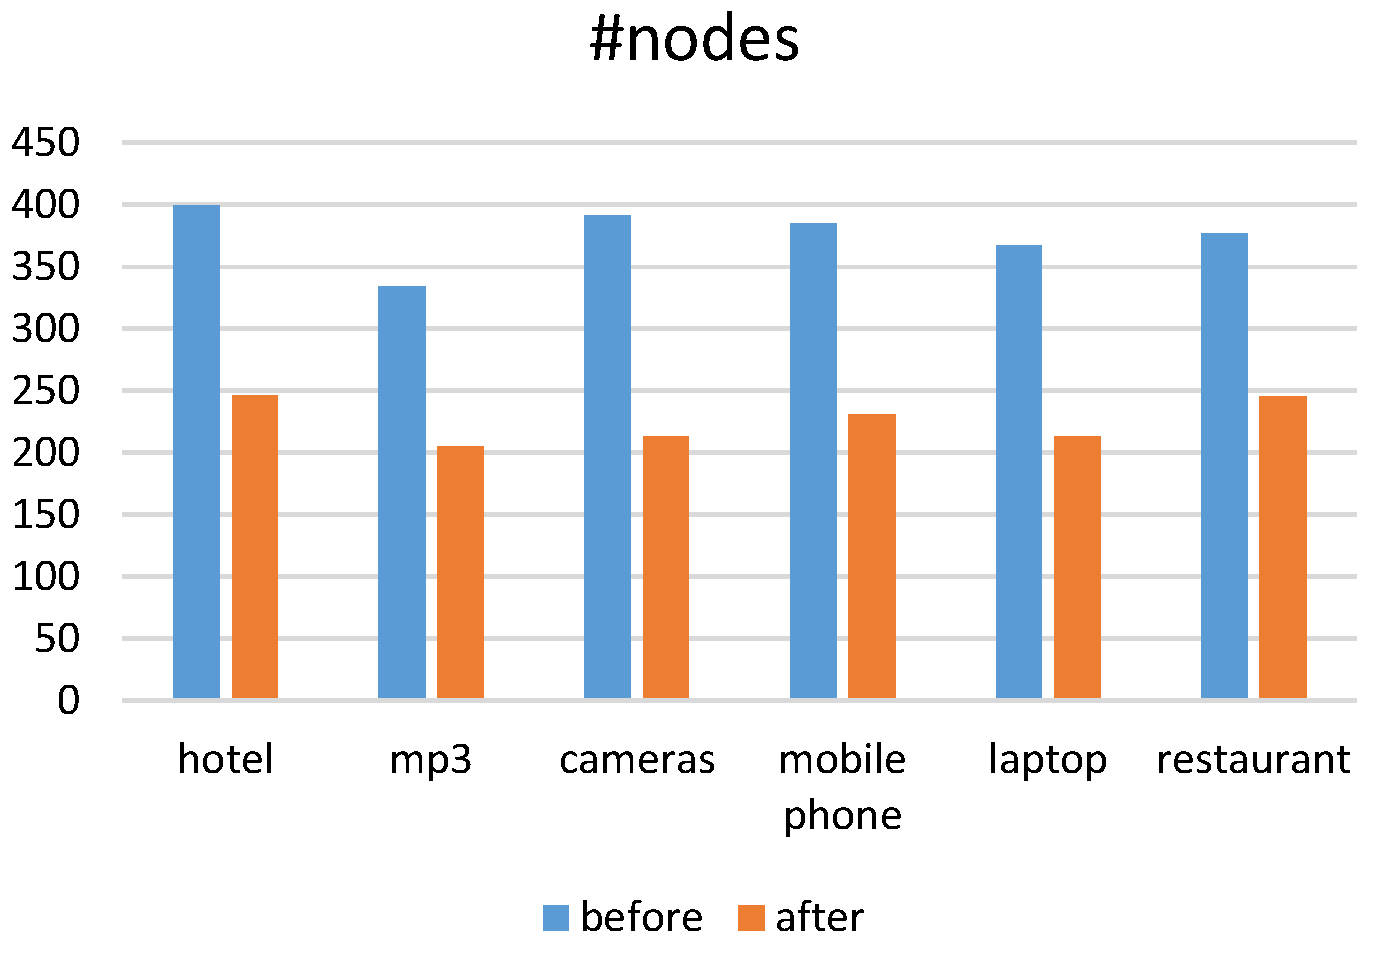
\includegraphics[width=0.48\columnwidth]{figures/1.pdf}
	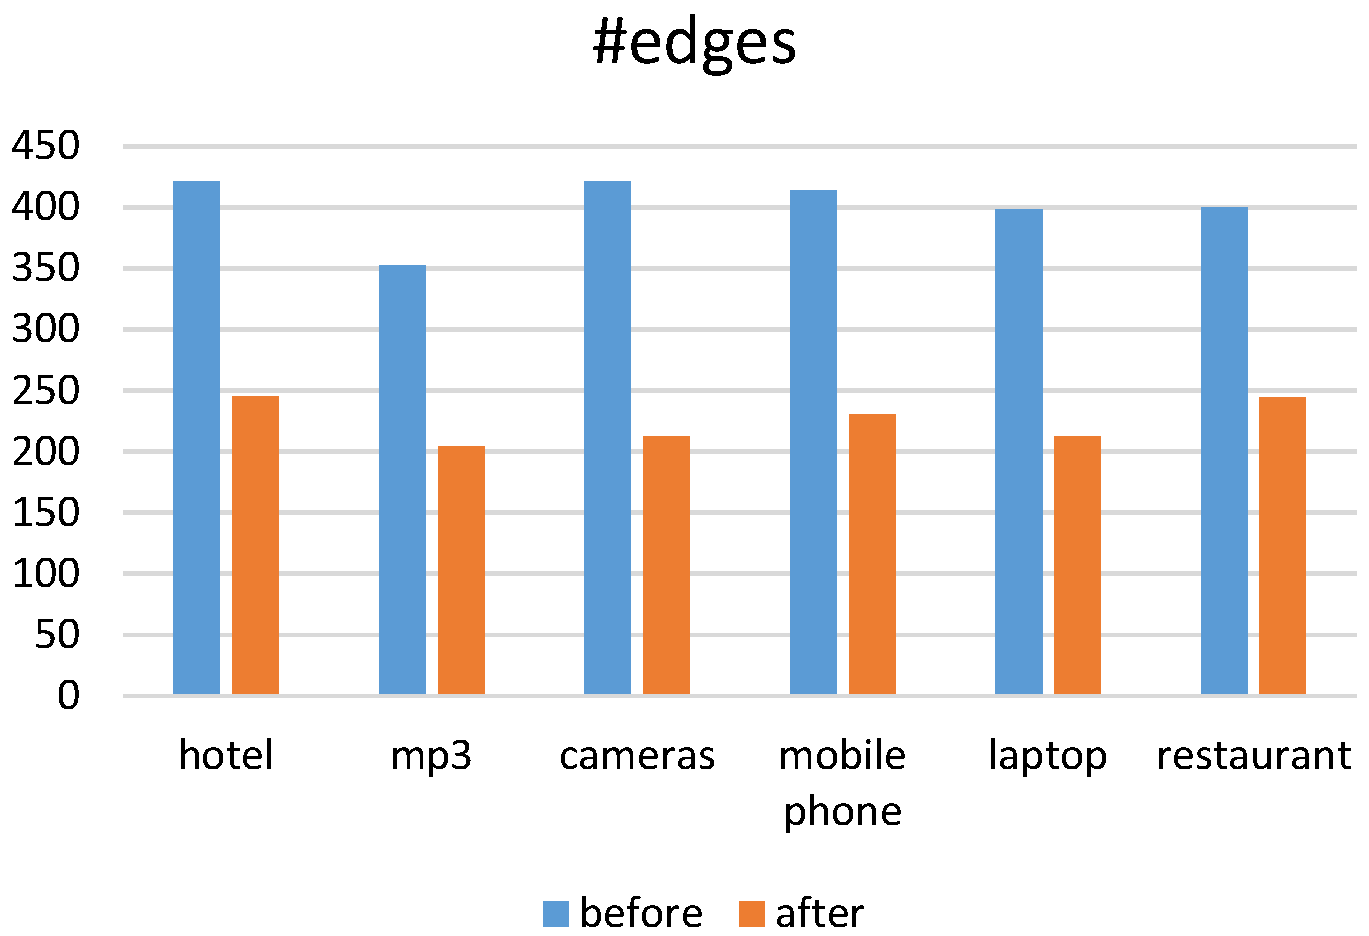
\includegraphics[width=0.48\columnwidth]{figures/2.pdf}
	\caption{Statistics of induced aspect taxonomy before and after taxonomy minimization}
	\label{fig:size}
%	\vspace{-10pt}
\end{figure}

Next, we evaluate our model as well as above baselines on the evaluation dataset described above.
We did not remove the duplicate aspect labels for the qualitative evaluation, 
since the repeated aspects are assume to be better.
%Because there are duplicates in the label set, aspect terms that are repeated are assume to be better. 
%The labels provided by the annotators are aggregated together without removing duplicated words, so we have 25 words in total.
%This is to ensure that the information about the different importances of aspects is preserved.
%When evaluating the models, 
%we compare the 5 aspect words generated by the models with those provided 
%by the annotators. 
For a given category, we first calculate the percentage of the 25 labels that exactly match one of the 5 aspect terms generated by the model 
as the \textit{hard accuracy} 
%(i.e. the first line for each category in \tabref{tab:comparison}) 
of the model. 
Formally, $Aspects(m) = [a_1, a_2, a_3, a_4, a_5]$ denotes 
the five prominent aspects generated from model $m$ for 
the given category.
$L = [l_1, l_2, ..., l_{25}]$ are the 25 golden aspect terms,
where $L^{(h)}= [l_{5h-4}, ..., l_{5h}]$ are from the $h$-th human annotator.
The hard accuracy is defined as:
\begin{equation}
	hacc(m) = \frac{\sum_{i=1}^{25}{hit(Aspects(m), l_i)}}{25}
\end{equation}
\begin{equation}
hit(Aspects(m), l_i) = 
\begin{cases}
1, & l_i \in Aspects(m) \\
0, & \text{otherwise, }
\end{cases}
\end{equation}
%We show the comparison results in \tabref{table:comparison}.
%Formally, 
%$Aspects(m, c) = [a_1, a_2, a_3, a_4, a_5]$ denotes the $5$ 
%prominent aspects generated from model $m$ given the category $c$.
%$[l_1, l_2, ..., l_{25}]$ is the 25 ground-truths annotated by
%humans. 
%We formulate the hard accuracy measure as follows:
%\begin{equation}
%hacc(m, c) = \frac{\sum_{i=1}^{25}{hit(Aspects(m, c), l_i)}}{25}
%\end{equation}
%\begin{equation}
%hit(Aspects(m, c), l_i) = 
%\begin{cases}
%1 &  \text{, if $l_i\in Aspects(m, c)$} \\
%0 &  \text{, otherwise}
%\end{cases}
%\end{equation}
%We formulate the hard accuracy measure as follows.
%$Aspects(m, c) = [a_1, a_2, a_3, a_4, a_5]$ denotes the $5$ 
%prominent aspects generated from model $m$ given the category $c$.
%$[l_1, l_2, ..., l_{25}]$ is the 25 ground-truths annotated by
%humans.

However, counting the number of exact matches 
makes the accuracy score discrete and coarse. 
Besides, it penalizes aspect terms that don't match the label
but actually have similar meanings.
%To remedy this, we use the semantic similarity between
%terms as a \emph{soft accuracy}  measure which is
%computed as follows.
To remedy this, we propose the \emph{soft accuracy}  evaluation measure.
For each set of five golden labels from 
$h$-th annotator, we first align each generated aspect $a_k \in Aspects(m)$
with one golden aspect $l_j \in L^{(h)}$ (i.e. $align^{(h)}(a_{k})=l_{j}$). 
We align the exact match terms together, and then choose the optimal alignment for the others by permuting all possible alignments. 
The optimal alignment $align^{(h)}(a_k)$ acheives maximum soft accuracy.
Then we calculate the soft matching score between
$Aspects(m)$ and $L^{(h)}$ as $\sum_{k=1}^{K}sim(a_{k}, align^{(h)}(a_k))$,
where $sim$ is the cosine similarity computed by 
Glove~\shortcite{pennington2014glove}
\footnote{ We use the GloVe embeddings 
	with 300 dimensions, trained from 840B tokens using common crawl data. }. 
We then compute the soft accuracy measure as follows:
%We sum such soft matching scores to represent the accuracy of the model. We then average such accuracies on 5 sets of labels from the 5 annotators as the soft accuracy measure:
\begin{equation}
sacc(m) =\frac{1}{5}*\sum_{h=1}^{5}\sum_{k=1}^{K}sim(a_k, align^{(h)}(a_k)), 
\end{equation}
where $K=5$ in this case.
The comparison results are shown 
in \tabref{table:comparison}. 

Our model (ExtRA) outperforms all the other baselines 
in all categories except cameras using the hard accuracy measure.
Besides, ExtRA is the best model on four out of six products under the 
soft accuracy measure. As shown in \tabref{synsetmatching}, the accuracy for
synset matching is relatively low for cameras and restaurant,
resulting in the lower accuracy in overall aspect extraction.

%\begin{figure*}[t!]
%\centering
%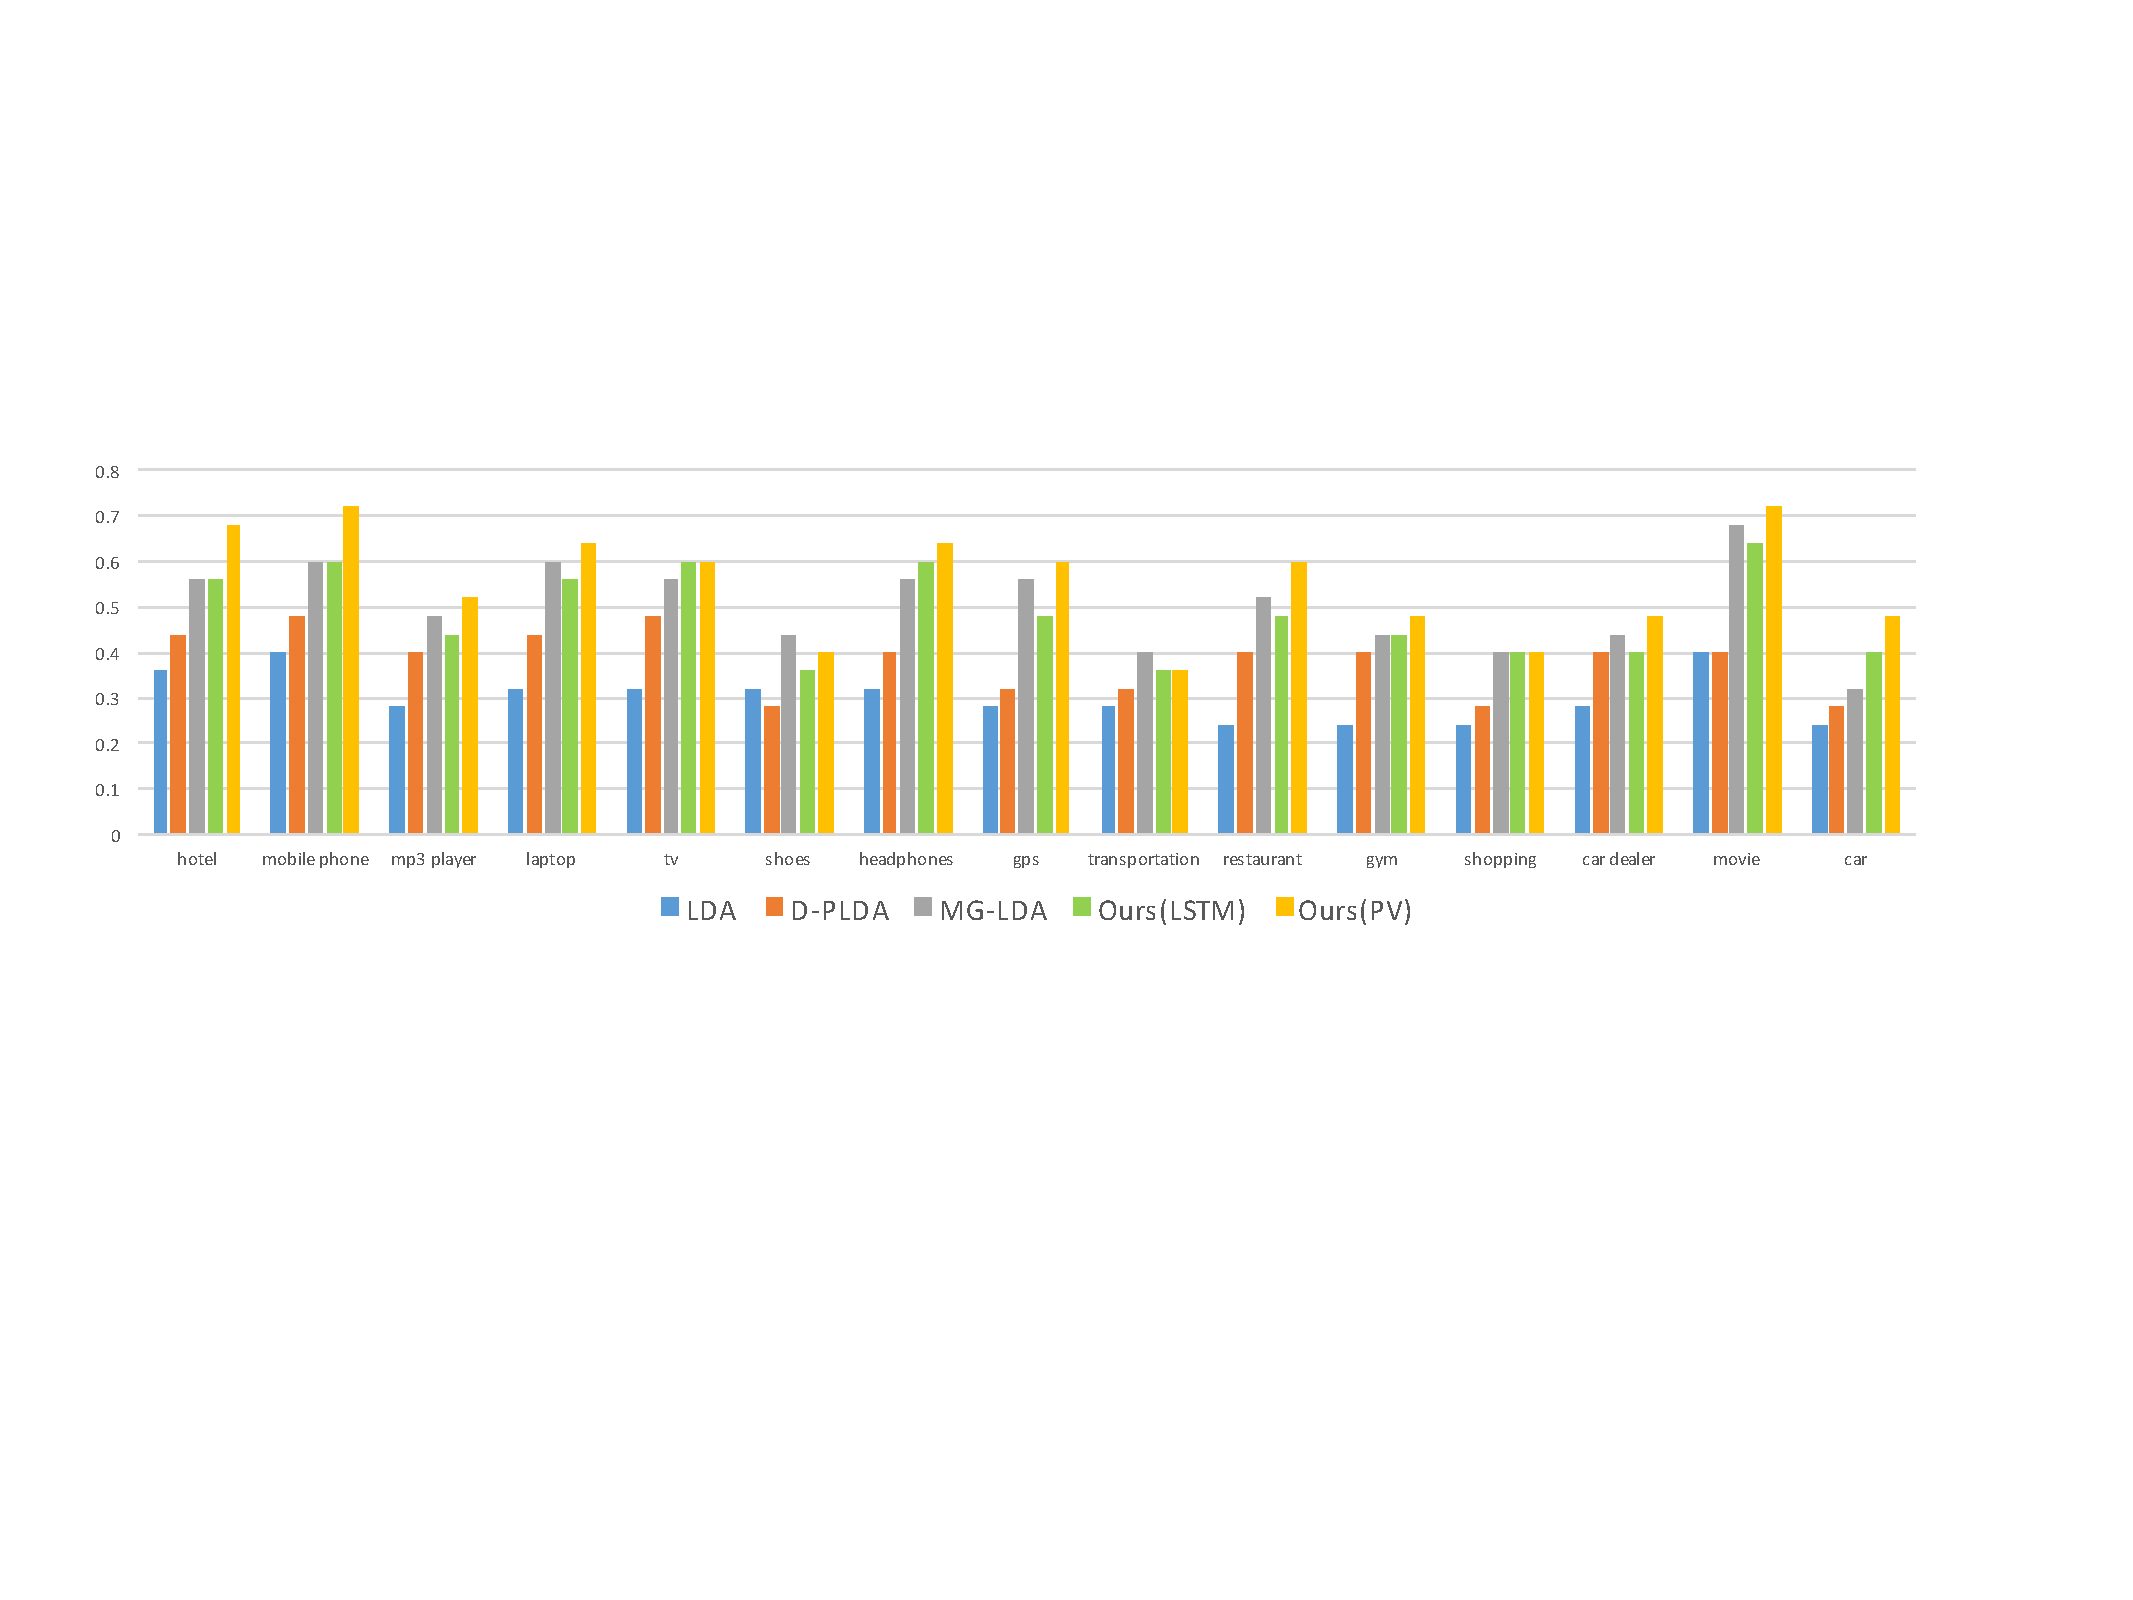
\includegraphics[width=2.0\columnwidth]{figures/results}
%\caption{Comparison of accuracies from different models on aspect extraction.}
%\label{fig:results}
%\end{figure*}  
\begin{table}[t]
	\scriptsize
	\centering
	\caption{Comparison of \emph{hard} (upper row) \& \emph{soft} (lower row) accuracies using different models for aspect extraction.}
	\label{table:comparison}
\begin{tabular}{|p{0.8cm}<{\centering}|c|c|c|c|c|c|}
	\hline
	&    LDA  & BTM &  \begin{tabular}[c]{@{}l@{}}MG-\\LDA \end{tabular}  & ABAE & AmodExt & ExtRA \\ \hline \hline
	\multirow{2}{*}{hotel}  & 0.16 & 0.16 & 0.16  & 0.16   & 0.44 & \textbf{0.56} \\ \cline{2-7} 
	&  0.50 & 0.49 & 0.67& 0.35  & 0.65  &  \textbf{0.70} \\ \hline
	\multirow{2}{*}{mp3}  & 0.0 & 0.08 & 0.08  & 0.0 & 0.35 &  \textbf{0.44} \\ \cline{2-7} 
	&   0.47 & 0.49 & 0.47 & 0.32 & 0.58 &  \textbf{0.60} \\ \hline
	\multirow{2}{*}{camera}  & 0.24 &\textbf{0.40}  & 0.28& 0.04 & 0.04  &  0.32 \\ \cline{2-7} 
	&   0.56 & \textbf{0.69} & 0.54 & 0.29 & 0.41  & 0.55 \\ \hline
	\multirow{2}{*}{\begin{tabular}[c]{@{}l@{}}mobile\\ phone\end{tabular}}  & 0.16 & 0.0 & 0.28 & 0.0  & 0.52 &  \textbf{0.60}  \\ \cline{2-7} 
	&   0.58 & 0.33 & 0.58 & 0.31 & \textbf{0.73}  & 0.71 \\ \hline
	\multirow{2}{*}{laptop}   & 0.08 & 0.24 & 0.24& 0.0 & 0.24  &  \textbf{0.28} \\ \cline{2-7} 
	&   0.40 & 0.50 & 0.50& 0.22 & 0.51  &  \textbf{0.53} \\ \hline
	\multirow{2}{*}{restaurant}  & 0.20 & 0.0 &0.0 & 0.0  & \textbf{0.56} & \textbf{0.56} \\ \cline{2-7} 
	&   0.49 & 0.38 & 0.42& 0.29 & \textbf{0.77}  & 0.72 \\ \hline
\end{tabular}

\end{table}

\begin{table}[th]
	\scriptsize
	\centering
	\caption{The five prominent aspect terms}
	\label{table:aspect_words}
	\begin{tabular}{|p{0.8cm}<{\centering}|p{0.79cm}<{\centering}|p{4.83cm}|}
		\hline
		\multirow{6}{*}{hotel} & LDA     & room, pool, stay, good, nice                           \\ \cline{2-3} 
		& BTM     & walk, good, room, stay, check                          \\ \cline{2-3} 
		& MGLDA   & room, stay, good, location, staff                      \\ \cline{2-3} 
		& ABAE    & shouted, room, terrific, accommodation, alexanderplatz \\ \cline{2-3} 
		& AmodExt & room, \textit{location, place}, view, staff                     \\ \cline{2-3} 
		& \textbf{ExtRA}   & \textbf{room, location, view, staff, service}                   \\ \hline
		\multirow{6}{*}{mp3}      & LDA     & work, great, good, music, ipod                         \\ \cline{2-3} 
		& BTM     & battery, ipod, work, song, good                        \\ \cline{2-3} 
		& MGLDA   & battery, ipod, music, song, good                       \\ \cline{2-3} 
		& ABAE    & documentation, content, portability, bought, table     \\ \cline{2-3} 
		& AmodExt & drive, quality, sound, feature, device                 \\ \cline{2-3} 
		& \textbf{ExtRA}   & \textbf{drive, sound\_quality, feature, screen, software}       \\ \hline
		\multirow{6}{*}{cameras}      & LDA     & lens, picture, buy, video, mode                        \\ \cline{2-3} 
		& BTM     & battery, picture, function, lens, good                 \\ \cline{2-3} 
		& MGLDA   & battery, picture, good, mpcture, mode                  \\ \cline{2-3} 
		& ABAE    & toy, picture, mailed, ultrazoom, sharpness             \\ \cline{2-3} 
		& AmodExt & \textit{picture, photo}, quality, feature, shot                 \\ \cline{2-3} 
		& \textbf{ExtRA}   & \textbf{image\_quality, photograph, feature, shot, lens}        \\ \hline
		\multirow{6}{*}{\begin{tabular}[c]{@{}l@{}}mobile\\ phone\end{tabular}}      &    LDA   & battery, buy, good, apps, work                         \\ \cline{2-3} 
		&    BTM     & core, good, work, para, apps                           \\ \cline{2-3} 
		&     MGLDA    & work, battery, screen, good, card                      \\ \cline{2-3} 
		&     ABAE    & cracked, amazing, continuously, archive, bought        \\ \cline{2-3} 
		&    AmodExt     & feature, screen, price, camera, quality                \\ \cline{2-3} 
		&    \textbf{ExtRA}     & \textbf{feature, price, screen, quality, service}               \\ \hline
		\multirow{6}{*}{laptop}      &    LDA     & screen, good, buy, drive, chromebook                   \\ \cline{2-3} 
		&    BTM   & windows, screen, work, drive, good                     \\ \cline{2-3} 
		&    MGLDA  & windows, battery, screen, good, year                   \\ \cline{2-3} 
		&    ABAE    & salign, returned, affordable, downloads, position      \\ \cline{2-3} 
		&     AmodExt & drive, machine, price, screen, life                    \\ \cline{2-3} 
		&   \textbf{ExtRA}  & \textbf{drive, price, screen, deal, performance}                \\ \hline
		\multirow{6}{*}{restaurant}      &    LDA     & food, good, room, time, great                          \\ \cline{2-3} 
		&  BTM       & good, room, pour, time, order                          \\ \cline{2-3} 
		& MGLDA     & great, good, place, time, make                         \\ \cline{2-3} 
		& ABAE    & jones, polite, told, chickpea, place                   \\ \cline{2-3} 
		& AmodExt    & food, service, place, experience, price                \\ \cline{2-3} 
		&  \textbf{ExtRA} & \textbf{service, food, experience, company, price}              \\ \hline
	\end{tabular}
%	\vspace{-0.3cm}
\end{table}

%\ZY{Our approach alleviate the overlapping problem by using the aspect  taxonomy.}

\subsubsection{Qualitative Analysis}
To qualitatively evaluate different models,
we present the extracted 5 aspect terms by each model from each domain in \tabref{table:aspect_words}. 
Our model (ExtRA) has significant advantage over other baselines for that we can do better aspect extraction with reasonable results, and extract not only words but also phrases as prominent aspects, \textit{e.g. sound quality, image quality}. The proposed model avoid the overlapping aspects appeared in our strong baseline (AmodExt) by deduplication using generated aspect taxonomy information. The overlapping aspects are marked in italics. For example, both \textit{location} and \textit{place} are extracted as top aspects, but they mean nearly the same concept. The results from other baseline methods, inevitably contain some sentiment words and opinions, like \textit{good, nice, great, etc.} Our model resolves such drawback by extracting aspect candidates from only nouns and using syntactic rules to find words that are frequently modified by adjectives.



%To evaluate the effect of different number of expected aspects, i.e. $K$, which 
%determines the coverage covered by expected aspects,
%we ask our annotators to provide different number of labels on two categories. 
%$K$ ranges from three to seven. 
%The performance of the four models when changing the number of aspects are shown in \figref{fig:differentk}. 
%It can be seen that our models can well extract aspects with variant coverage and perform constantly better than all other models regardless of the number of expected aspects. 


%As shown in \tabref{table:rankingeffect},
%we find that: 1) our proposed semantic similarity score for ranking words is indeed effective; 2) the word importance decreasing mechanism improves the prominence of the extracted aspect term.

%the final setup which uses word ranking method 
%cooperated with duplicate prevention
%outperforms others with a substantial margin 
%on all categories.
%has clear advantage across all product categories.

